% metrics-test.tex — Test document for metrics.lua v3.0
\documentclass[11pt, a4paper]{scrartcl}
\usepackage{swarmbeauty}

\title{Metrics Lua Test}
\subtitle{Verifying metrics.lua v3.0}
\author{Programmer Agent}
\date{May 14, 2026}

% Load metrics module
\directlua{dofile("../lua/metrics.lua")}

\begin{document}

\swarmtitlepage

\section{First Section}
Some text here with a figure and table. This section should be counted.

\begin{figure}[H]
  \centering
  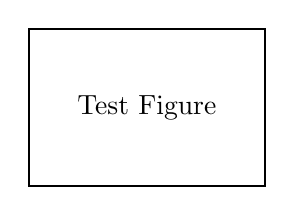
\begin{tikzpicture}
    \draw[thick] (0,0) rectangle (3,2);
    \node at (1.5,1) {Test Figure};
  \end{tikzpicture}
  \caption{A test figure}
\end{figure}

\subsection{Subsection One}
This subsection tests subsection counting.

\section{Second Section}
More text content here for word counting.

\begin{table}[H]
  \centering
  \begin{tabular}{l c}
    \swarmtoprule
    Item & Value \\
    \swarmmidrule
    Alpha & 1 \\
    Beta & 2 \\
    \swarmbottomrule
  \end{tabular}
  \caption{A test table}
\end{table}

\section{Third Section}
Final section with some math: $E = mc^2$.
\label{eq:einstein}

\begin{noteblock}
This document is testing the metrics.lua v3.0 script with file inclusion
tracking, structure counters, and word count estimation.
\end{noteblock}

\end{document}
